\documentclass[crop,tikz]{standalone}
\usepackage{tkz-euclide}
\usetikzlibrary{arrows.meta}
\usetkzobj{all}
\usetikzlibrary{shapes}


\tikzstyle{myarrows}=[line width=1mm,draw=blue,-triangle 45,postaction={draw, line width=3mm, shorten >=4mm, -}]
\begin{document}

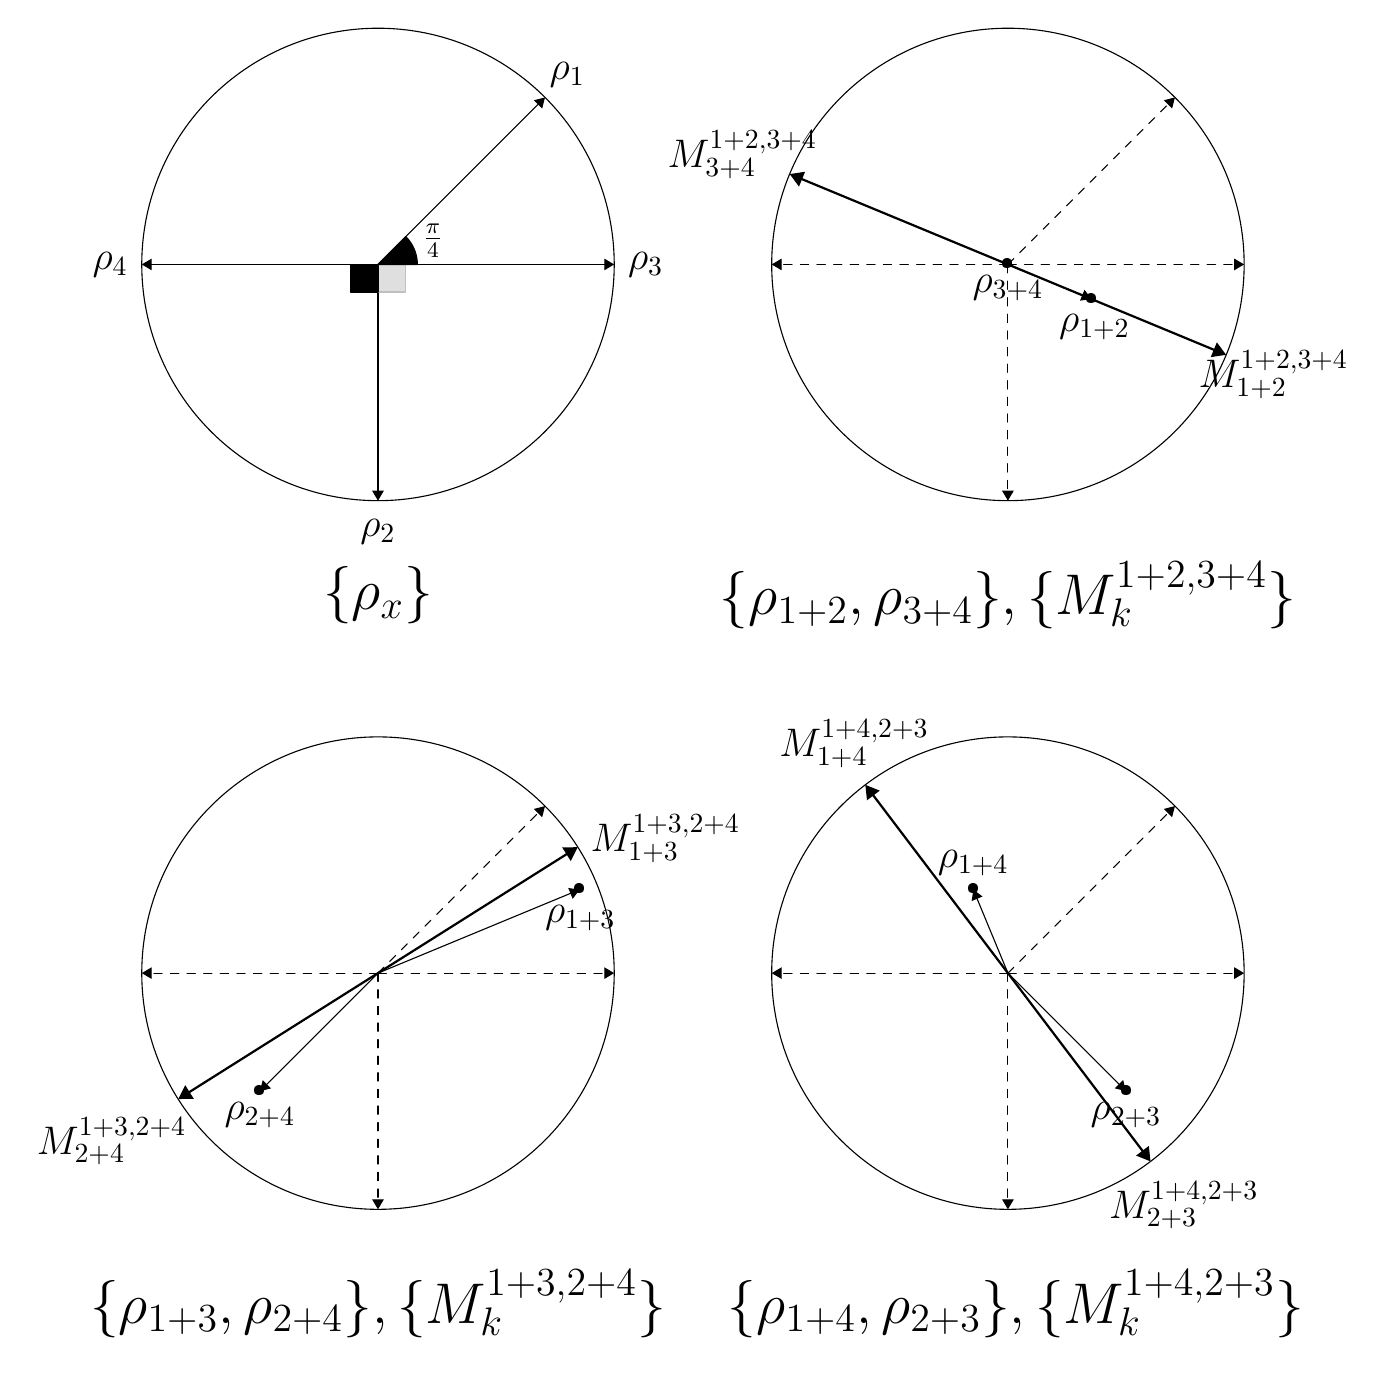
\begin{tikzpicture}[line cap=round, line join=round, >=Triangle]

\begin{scope}[ shift={(0,0)}]
\draw  (0,0) ellipse (3 and 3);

\begin{scope}[rotate=-45]    
\draw[->]  (0,0) -- (0,3);
\draw (0,3.4) node {\Large $\rho_1$};
\end{scope}

\begin{scope}[rotate=180]    
	\draw[->]  (0,0)  -- (0,3);
	\draw (0,3.4) node {\Large $\rho_2$};
\end{scope}

\begin{scope}[rotate=270]    
	\draw[->]  (0,0)  -- (0,3);
	\draw (0,3.4) node {\Large $\rho_3$};
\end{scope}

\begin{scope}[rotate=90]    
	\draw[->]  (0,0)  -- (0,3);
	\draw (0,3.4) node {\Large $\rho_4$};
\end{scope}




\draw [shift={(0,0)},lightgray, fill, fill opacity=0.5] (0,0) rectangle (0.35,-0.35);
\draw [shift={(0,0)}, fill] (0,0) rectangle (-0.35,-0.35);

\draw [shift={(0,0)}, fill] (0,0) -- (45:0.5) arc (45:0:0.5) -- cycle;
\node at (0.7,0.3) {\large $\frac{\pi}{4}$};
\node at (0,-4.2) {\huge $\{\rho_x\}$ };
\end{scope}



\begin{scope}[ shift={(8,0)}] 
\begin{scope}[rotate=-45]    
\draw[->, dashed]  (0,0) -- (0,3);
\end{scope}

\begin{scope}[rotate=180]    
	\draw[->, dashed]  (0,0)  -- (0,3);
\end{scope}

\begin{scope}[rotate=270]    
	\draw[->, dashed]  (0,0)  -- (0,3);
\end{scope}

\begin{scope}[rotate=90]    
	\draw[->, dashed]  (0,0)  -- (0,3);
\end{scope}	
	\draw[->]  (0,0)  -- (1.0605,-0.4392);
	\node at (1.0605,-0.4392) {\textbullet};
	\draw (1.1,-0.8) node {\Large $\rho_{1+2}$};
	
	\begin{scope}[rotate=-112.5000]
 	\draw[->,thick]  (0,0)  -- (0,3);
 	\draw  (0,3.65) node {\Large $M^{1+2,3+4}_{1+2}$};
 	\end{scope}
 	
 	\begin{scope}[rotate=67.5000]
 	\draw[->,thick]  (0,0)  -- (0,3);
 	\draw  (0,3.65) node {\Large $M^{1+2,3+4}_{3+4}$};
 	\end{scope}
 	
 	\node at (0,0) {\textbullet};
	\draw (0,-0.3) node {\Large $\rho_{3+4}$};
	\draw  (0,0) ellipse (3 and 3);
	\node at (0,-4.2) {\huge $\{\rho_{1+2},\rho_{3+4}\},\{M^{1+2,3+4}_k\}$ };
\end{scope}

\begin{scope}[ shift={(8,-9)}] 
\begin{scope}[rotate=-45]    
\draw[->, dashed]  (0,0) -- (0,3);
\end{scope}

\begin{scope}[rotate=180]    
	\draw[->, dashed]  (0,0)  -- (0,3);
\end{scope}

\begin{scope}[rotate=270]    
	\draw[->, dashed]  (0,0)  -- (0,3);
\end{scope}

\begin{scope}[rotate=90]    
	\draw[->, dashed]  (0,0)  -- (0,3);
\end{scope}	
	\draw[->]  (0,0)  -- (-0.4393,1.0607);
	\node at (-0.4393,1.0607) {\textbullet};
	\draw (-0.4393,1.4) node {\Large $\rho_{1+4}$};
	
	\begin{scope}[rotate=37.1388]
 	\draw[->,thick]  (0,0)  -- (0,3);
 	\draw  (0.2,3.5) node {\Large $M^{1+4,2+3}_{1+4}$};
 	\end{scope}
 	
 	\begin{scope}[rotate=180+37.1388]
 	\draw[->,thick]  (0,0)  -- (0,3);
 	\draw  (-0,3.7) node {\Large $M^{1+4,2+3}_{2+3}$};
 	\end{scope}
 	
 	
 	\draw[->]  (0,0)  -- ( 1.5,-1.5);
 	\node at (1.5,-1.5) {\textbullet};
	\draw (1.5,-1.8) node {\Large $\rho_{2+3}$};
	\draw  (0,0) ellipse (3 and 3);
	\node at (0.1,-4.2) {\huge $\{\rho_{1+4},\rho_{2+3}\},\{M^{1+4,2+3}_k\}$ };
\end{scope}









\begin{scope}[ shift={(0,-9)}] 
\begin{scope}[rotate=-45]    
\draw[->, dashed]  (0,0) -- (0,3);
\end{scope}

\begin{scope}[rotate=180]    
	\draw[->, dashed]  (0,0)  -- (0,3);
\end{scope}

\begin{scope}[rotate=270]    
	\draw[->, dashed]  (0,0)  -- (0,3);
\end{scope}

\begin{scope}[rotate=90]    
	\draw[->, dashed]  (0,0)  -- (0,3);
\end{scope}	
	\draw[->]  (0,0)  -- ( 2.5607,1.0607);
	\node at (2.5607,1.0607) {\textbullet};
	\draw (2.57,0.7) node {\Large $\rho_{1+3}$};
	
	\begin{scope}[rotate=-57.7644]
 	\draw[->,thick]  (0,0)  -- (0,3);
 	\draw  (0.5,4) node {\Large $M^{1+3,2+4}_{1+3}$};
 	\end{scope}
 	
 	\begin{scope}[rotate=180-57.7644]
 	\draw[->,thick]  (0,0)  -- (0,3);
 	\draw  (-0,4) node {\Large $M^{1+3,2+4}_{2+4}$};
 	\end{scope}
 	
 	
 	\draw[->]  (0,0)  -- ( -1.5,-1.5);
 	\node at (-1.5,-1.5) {\textbullet};
	\draw (-1.5,-1.8) node {\Large $\rho_{2+4}$};
	\draw  (0,0) ellipse (3 and 3);
	\node at (0,-4.2) {\huge $\{\rho_{1+3},\rho_{2+4}\},\{M^{1+3,2+4}_k\}$ };
\end{scope}
\end{tikzpicture}

\end{document}